\documentclass[a4paper, 12pt, one column]{article}

\usepackage[english]{babel}
\usepackage[utf8x]{inputenc}
\usepackage[T1]{fontenc}
\usepackage{tikz}
\usepackage{xcolor}
\usepackage{subfig}
\usepackage{caption}
\usepackage{float}
%\usepackage[top=1.3cm, bottom=2.0cm, outer=2.5cm, inner=2.5cm, heightrounded,
%marginparwidth=1.5cm, marginparsep=0.4cm, margin=2.5cm]{geometry}
\usepackage{graphicx} 
\usepackage{hyperref} 
\usepackage{amsmath} 
\usepackage{amsfonts}
\usepackage{amssymb} 
\usepackage{multirow}
\usepackage{eurosym}
\usepackage{booktabs}
\usepackage{algorithm}
\usepackage{algorithmic}
\usepackage{wrapfig}
\usepackage{blkarray}
%\usepackage{pdfpages}
\usepackage{listings}
\usepackage[nameinlink]{cleveref}
\crefdefaultlabelformat{#2#1#3}
\graphicspath{{images/}}



\newcommand{\hsp}{\hspace{11pt}}
\newcommand{\HRule}{\rule{\linewidth}{0.5mm}}

\graphicspath{{images/}}


\begin{document}

\begin{titlepage}
  \begin{sffamily}
  \begin{center}

    \begin{figure}[h]
	    
\includegraphics[width=4cm]{logo_esilv_png_blanc.png}\hfill
	\end{figure}  	
	
    \vspace{2cm}
    \textsc{\LARGE Advanced Machine Learning}\\[0.5cm]
    \vspace{2cm}

  %  \textsc{\Large }\\[1.5cm]

    % Title
    \HRule \\[0.4cm]
    { \huge \bfseries Project Report}
    \HRule \\[0.4cm]

    \vspace{3cm}

  \end{center}
  % Author and group
    \begin{minipage}{0.4\textwidth}
      \begin{flushleft} \large
		\textbf{\textit{Students :}} \\        
        \textsc{KUOCH Jacky}\\
        \textsc{NICOLAS Kevin}\\
        \textsc{ALIZADEH Charly}\\
        \textsc{LIMNAVONG Thomas}\\
      \end{flushleft}
    \end{minipage}
    
    \begin{minipage}{0.9\textwidth}
      \begin{flushright} \large
        \textsc{DIA 1}\\
      \end{flushright}
      
    \end{minipage}
  
  \end{sffamily}
\end{titlepage}


\renewcommand{\headrulewidth}{1pt}
\fancyhead[H]{Advanced Machine Learning}
\fancyhead[R]{Project}
\fancyhead[L]{
\includegraphics[scale=0.2]{logo_esilv_png_blanc.png}}
\fancyfoot[C]{\thepage}


\section*{Subject}

On the course module folder you will find a dataset listing purchase transactions. Adapt to the capacity of your computer (work on sampling possible).
The objective is to model the income (transactionRevenue) generated per person (fullVisitorId).

The challenge is not to have the best performance but on the contrary to have the most thoughtful and structured approach to address the problem
The data was uploaded on October 26 and the assignment is due on Monday December 20 at 11:59 p.m. at the latest
The project is to be carried out in teams of 4 maximum.

Your report will contain :\\

\begin{itemize}
    \item \textbf{Your analysis of the problem, the data, the description of your approach to solve it, the algorithms tested, their results in terms of performance and the importance of the variables (At least 3 algorithmic approaches required).
    \item Models you tried and how you tuned them. Your best prediction evaluation.
    \item Your assessment on the best way to solve the problem and the new avenues that you could test with more time.
    \item Format: Word or PowerPoint version, a PDF if other writing format.
    \item 4 or 5 pages minimum, as explicit as possible: as if you were returning it to your business client within the company.}
\end{itemize}


\newpage

\section{Problem Analysis}

The problem we are facing is a regression one, meaning that we need to predict a continuous target. The features are both continuous and categorical, for the categorical features we'll need to convert them to numerical features by using dummy/indicator variables. 

\newpage

\section{Data Analysis}

Our dataset contains 55 columns and 903.653 rows. As we are studying purchase  
transactions, we have information like the date and time of the purchase, the location of it but also the browser or operation system on which the transaction took place. 

\subsection{Location}
As consumption trends may vary a lot according to the regions of the world but also meet depending on communities' affinities, it is important to consider the various locations that our data offers us when trying to study the behaviours behind purchase transactions.

Let's have a look at the continents, subcontinents, countries and cities of our transactions. We will start by studying on a global scale and observe the number of transactions per continents: 

\begin{center}
\begin{tabular}{ |c|c| } 
 \hline
 \textbf{Continent} & \textbf{Count} \\ 
 \hline
Americas & 450.377\\
Asia & 223.698\\
Europe & 198.311 \\
Oceania & 15.054 \\
Africa & 14.745 \\
(not set) & 1468 \\
 \hline
\end{tabular}
\end{center}

We easily see that our dataset offers a majority of American transactions as Americas' transactions numbers represent almost the double of transactions of the second continent most represented: Asia. Europe comes in third with a still relevant number of transactions before Oceania and Africa with numbers much lower than the three first continents.

\subsection{Digital tools}
We also have many information about the devices and tools used by the user to realize their transaction including the web browser, the operating system and if they are using their phone or their desktop. 

\begin{center}
\begin{tabular}{ |c|c| } 
 \hline
 \textbf{Browser} & \textbf{Count} \\ 
 \hline
Chrome & 620.364 \\
Safari & 182.245 \\
Firefox & 37.069 \\ 
Internet Explorer & 19.375 \\
Edge & 10.205 \\ 
... & .. \\
 \hline
\end{tabular}
\end{center}

\begin{center}
\begin{tabular}{ |c|c| } 
 \hline
 \textbf{Device} & \textbf{Count} \\ 
 \hline
Desktop & 664.479\\
Mobile & 208.725\\
Tablet & 30.449 \\
 \hline
\end{tabular}
\end{center}

\begin{center}
\begin{tabular}{ |c|c| } 
 \hline
 \textbf{Operating System} & \textbf{Count} \\ 
 \hline
Windows & 350.072\\
Macintosh & 253.938\\
Android & 123.892 \\
iOS & 107.665 \\
Linux & 35.034 \\
Chrome OS & 26.337 \\
(not set) & 4.695 \\
... & ... \\ 
 \hline
\end{tabular}
\end{center}

\begin{center}
\begin{tabular}{ |c|c| } 
 \hline
 \textbf{Source} & \textbf{Count} \\ 
 \hline
Google & 400.788\\
Youtube & 212.602\\
(direct) & 143.028 \\
mall.googleplex.com & 66.416 \\
Partners & 16.411 \\
... & ... \\ 
 \hline
\end{tabular}
\end{center}

Looking at this could explain to us which tools offer the best User Experiences and have more chance to convert a visit into a purchase. Nowadays, it is really difficult to guide a consumer through all the steps starting from the user reaching our platform, then having a look at our products, convince him to buy the product and then the final step, the payment. Many means are implemented so that the customer experience is as optimized as possible. \\

Therefore, knowing which browser, which operating system or the source where the customers come from is a a precious piece of information so that companies can invest in the fields where their customers are most likely to make a purchase.

\newpage

\section{Models}

\subsection{Cleaning the data}
Before applying our different algorithms, we had some cleaning to do on our data. First, we noticed that our target was missing a lot of values. We considered that these rows were visits that were not converted into transactions, therefore we set a 0 values for all the rows missing a target value.

We also made this assumption for the following columns:
\begin{itemize}
    \item isTrueDirect
    \item page
    \item adNetworkType
    \item newVisits
    \item bounces
    \item pageviews
\end{itemize}

Single-value columns are useless for machine learning therefore we dropped them.

We also dropped the following columns because we judged that they didn't contain pertinent informations, or because too much observations had them.
\begin{itemize}
    \item metro
    \item region
    \item city
    \item sessionId
    \item visitId
    \item adContent
    \item isVideoAd
    \item slot
    \item gclId
    \item keyword
    \item campaign
\end{itemize}


Then we converted the categorical columns into numerical's. Those columns are:
\begin{itemize}
    \item channelGrouping
    \item source
    \item medium
    \item continent
    \item subContinent
    \item country
    \item browser
    \item operatingSystem
    \item deviceCategory
    \item networkDomain
    \item referralPath
    \item isTrueDirect
    \item adNetworkType
\end{itemize}

We also converted the date column into DateTime python objects and extracted the day of the week and month, then we removed the date column.

\subsection{Feature Engineering}

Before grouping the dataset by the fullVisitorId we added one feature called timeSpanSinceFirstVisit which compute the time difference between the first time a user
visited the shop and the current visit of the shop.

When grouping the dataset by fullVisitorId we had to make choices for the aggregation of the different columns. You can find those aggregation choices in the \cref{tab:agg_functions}

\begin{table}[H]
\centering
\begin{tabular}{|l|l|}
    \hline
    \textbf{Feature} & \textbf{Aggregation function(s)}\\ \hline
    channelGrouping & max \\ \hline
    visitNumber & max \\ \hline
    visitStartTime & max \\ \hline
    source & last \\ \hline
    medium & last \\ \hline
    isTrueDirect & last \\ \hline
    referralPath & last \\ \hline
    hits & sum, 'mean', 'min', 'max', 'median' \\ \hline
    pageviews & sum, 'mean', 'min', 'max', 'median' \\ \hline
    bounces & sum, 'mean' \\ \hline
    newVisits & max \\ \hline
    transactionRevenue & sum \\ \hline
    continent & last \\ \hline
    subContinent & last \\ \hline
    country & last \\ \hline
    networkDomain & last \\ \hline
    browser & last \\ \hline
    operatingSystem & last \\ \hline
    isMobile & last \\ \hline
    deviceCategory & last \\ \hline
    page & last \\ \hline
    adNetworkType & last \\ \hline
    dayofweek & last \\ \hline
    month & last \\ \hline
    timeSpanSinceFirstVisit & last \\ \hline
\end{tabular}
\caption{Per column aggregation functions}
\label{tab:agg_functions}
\end{table}

\subsection{Split between train, val and test}

We split the dataset between train, val and test set using 80\%, 10\% and 10\% of the data respectively.
We used the function train_test_split from sklearn to have a similar distribution of the data between all the datasets.
We also scaled the all the dataset using the training set to fit the scaler (we used sklearn's MinMaxScaler with range between 0 and 1).
Finally we applied a last processsing to the training set by undersampling the observations with a target equal to 0 in order to have the
same amount of null and non null targets.


\subsection{Models}

\subsubsection{Random Forest}

First we trained a binary classifier to predict wether an observations have a null or non null target. To do so we used a random forest classifier.
You can find the results bellow.

\begin{table}[H]
\centering
\begin{tabular}{|l|l|}
    \hline
    577078 & 0\\ \hline
    1 & 8177\\ \hline
\end{tabular}
\caption{Confusion matrix for the train set}
\label{tab:cm_train}
\end{table}
\begin{table}[H]
\centering
\begin{tabular}{|l|l|}
    \hline
    14370 & 57\\ \hline
    134 & 71\\ \hline
\end{tabular}
\caption{Confusion matrix for the validation set}
\label{tab:cm_val}
\end{table}


\begin{table}[H]
\centering
\begin{tabular}{|l|l|}
    \hline
    Accuracy & F1\\ \hline
    0.99 & 0.99\\ \hline
\end{tabular}
\caption{Train scores}
\label{tab:train_scores}
\end{table}
\begin{table}[H]
\centering
\begin{tabular}{|l|l|}
    \hline
    Accuracy & F1\\ \hline
    0.99 & 0.43\\ \hline
\end{tabular}
\caption{Val scores}
\label{tab:val_scores}
\end{table}



\subsubsection{Feed Forward Neural Network}

Then we trained a neural network on the undersampled. You can find the evolution of the loss on \cref{fig:loss_reg} and a visualization of the model performance on 

\begin{figure}[H]
\centering
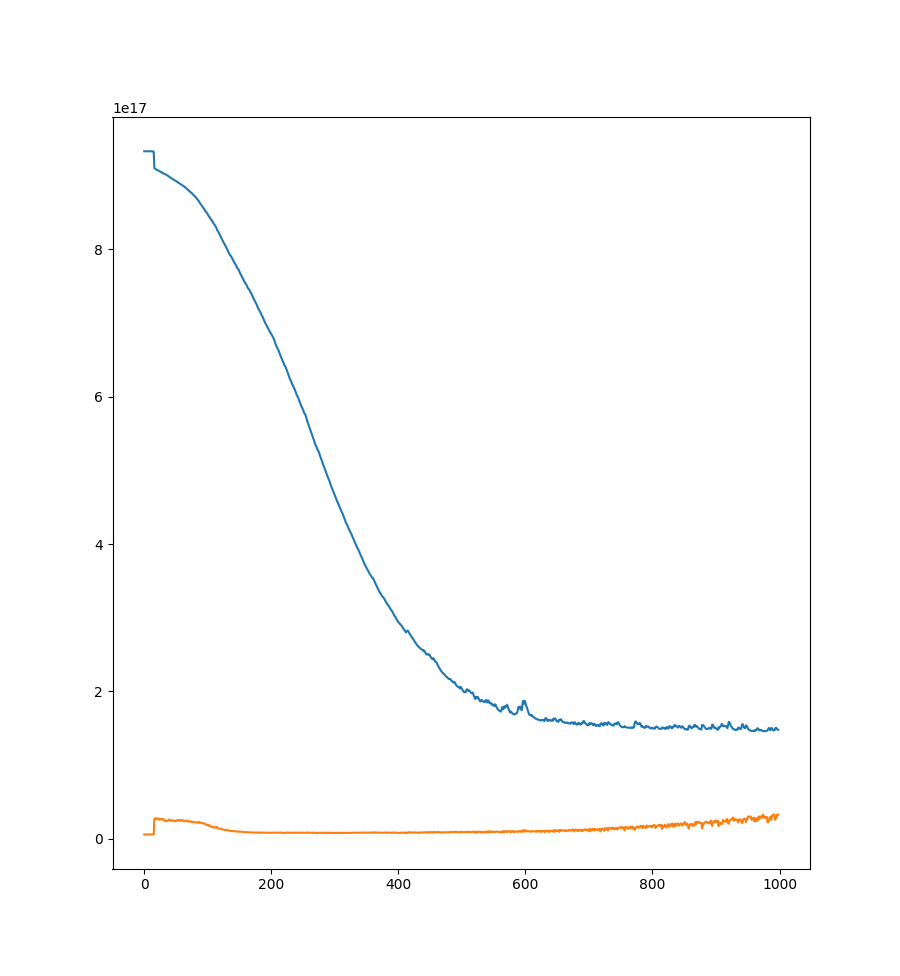
\includegraphics[scale=0.5]{loss_reg.png}
\caption{Evolution of the loss, in blue the training loss and in orange the validation loss}
\label{fig:loss_reg}
\end{figure}

\begin{figure}[H]
\centering
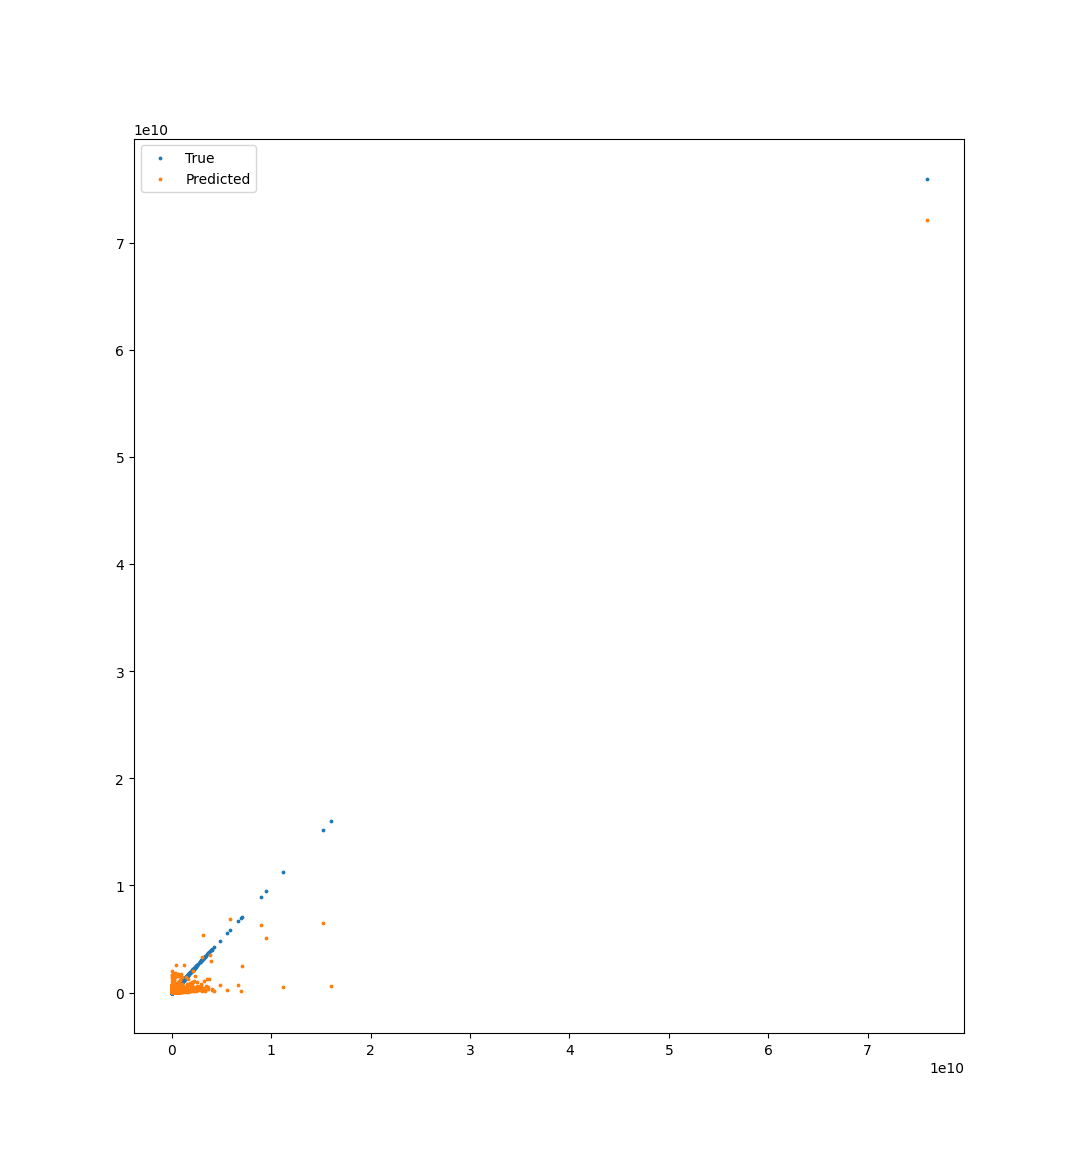
\includegraphics[scale=0.5]{train_target.png}
\caption{Train target visualization}
\label{fig:train_target}
\end{figure}

\begin{figure}[H]
\centering
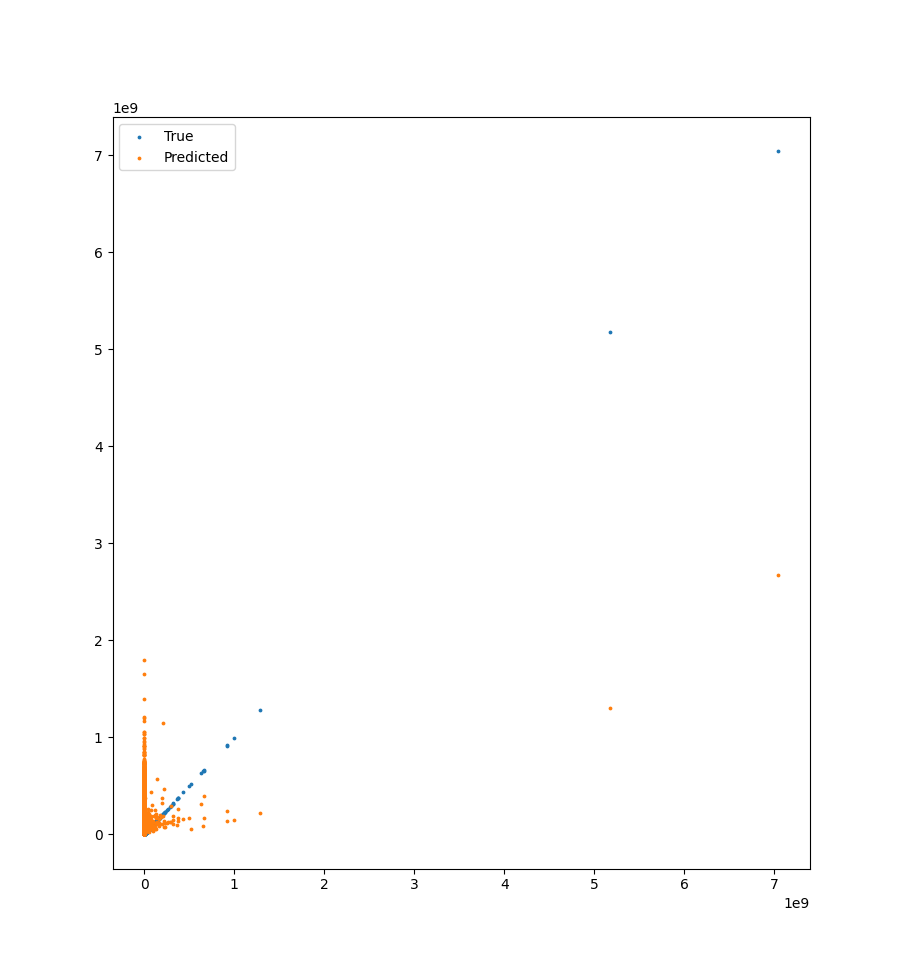
\includegraphics[scale=0.5]{val_target.png}
\caption{Val target visualization}
\label{fig:val_target}
\end{figure}

As you can see the model performs very badly, we tried to improve it but could achieve any improvement.

\subsection{Final model}

To predict the target we used both models. First we predict which observations will yield to a non null target using the random forest classifier, then we use the neural network to make prediction on those observations. You can find the R2 scores in

\begin{table}[H]
\centering
\begin{tabular}{|l|l|l|}
    \hline
    Train & Val & Test\\ \hline
    0.81 & 0.41 & 0.13 \\ \hline
\end{tabular}
\caption{R2 scores}
\label{tab:R2_scores}
\end{table}


\end{document}
